%!TEX TS-program = xelatex
\documentclass[12pt]{beamer}
% Add "aspectratio=169" to have wider slides

\usepackage{MacauMetropolis} % Colors and other styles

% This template uses the Metropolis theme by Matthias Vogelgesang (https://github.com/matze/mtheme). 


%-------------------------------------
% Title information
%-------------------------------------
\title{Macau Metropolis Theme}
\subtitle{An Unofficial \LaTeX \space Template for University of Macau}
\date{\today}
\author{Daina Chiba}
\institute{University of Macau}
\titlegraphic{\hfill
\includegraphics[height=2cm]{figures/UMlogo.png}} % Adds a logo 

%-------------------------------------
% Begin the document
%-------------------------------------
\begin{document}

\maketitle % Adds the title
%-------------------------------------
% Outline
%-------------------------------------
\begin{frame}[plain]{Outline} % "Plain" omits the page number
	\tableofcontents
	%\tableofcontents[hideallsubsections] % hide subsections
\end{frame} 


%===========================================================%
% Section 1: Building blocks
%===========================================================%

\section{Basic building blocks}


%~~~~~~~~~~~~~~~~~~~~~~~~~~~~~~~~~~~~~~~~~~~~~~~~%
\begin{frame}{{\color{UMYellow} Five colors} defined in the template}
\begin{columns}
	\column{0.35\linewidth}
    	\begin{figure}
        \centering
        
\includegraphics[height=3cm]{figures/UMlogo.png}
        \caption{UM Logo}
        \end{figure}
	\column{0.64\linewidth}
        \begin{itemize}
        \item {\color{UMBlue}\bf UMBlue} is the symbol color of the university.
        \item {\color{UMLightBlue}\bf UMLightBlue}
        \item {\color{UMYellow}\bf UMYellow}
		\item {\color{UMRed}\bf UMRed}
		\item {\color{UMGreen}\bf UMGreen}
        \end{itemize}
	\end{columns} 
\end{frame}
%~~~~~~~~~~~~~~~~~~~~~~~~~~~~~~~~~~~~~~~~~~~~~~~~%


%~~~~~~~~~~~~~~~~~~~~~~~~~~~~~~~~~~~~~~~~~~~~~~~~%
{
\setbeamercolor{background canvas}{bg=UMLightBlue}
\begin{frame}

 \color{UMYellow}{\bf\Large Use UMBlue as background color.}

\end{frame}
}
%~~~~~~~~~~~~~~~~~~~~~~~~~~~~~~~~~~~~~~~~~~~~~~~~%



%~~~~~~~~~~~~~~~~~~~~~~~~~~~~~~~~~~~~~~~~~~~~~~~~%
\begin{frame}{{\color{UMYellow} Highlighting} texts with blocks}

Four types of blocks are available:
\bigskip

\begin{columns}
	\column{0.49\linewidth}
		\begin{block}{}
		This is a block without a title. So there is no title in this block. This is a block without a title. So there is no title in this block. This is a block without a title. So there is no title in this block. 

		\end{block}
	\column{0.49\linewidth}
		\begin{block}{Block Title}
		A \emph{default} block with a title
		\end{block}

		\begin{alertblock}{Block Title}
		An \emph{alert} block with a title
		\end{alertblock}

\end{columns} 
		\begin{exampleblock}{Block Title}
		An \emph{example} block with a title
		\end{exampleblock}
\end{frame}
%~~~~~~~~~~~~~~~~~~~~~~~~~~~~~~~~~~~~~~~~~~~~~~~~%


%~~~~~~~~~~~~~~~~~~~~~~~~~~~~~~~~~~~~~~~~~~~~~~~~%
\begin{frame}{{\color{UMYellow} What you need} to typeset this template}

\begin{exampleblock}{Metropolis theme}
Available at {\footnotesize \href{https://github.com/matze/mtheme}{github.com/matze/mtheme}}	
\end{exampleblock}

\begin{exampleblock}{UM logo files}
\begin{itemize}
\item Available from \href{linktoUM}{UM's website} (internal access only)
\item Download the following two: 
	\begin{enumerate}
	\item \href{linktoUM}{\footnotesize {UMlogo.png}}
	\item \href{linktoUM}{\footnotesize {UMlogo\_footer.png}}
	\end{enumerate}
\item Save these logo files under the {\tt \footnotesize figures} directory located in the same directory that contains the .tex file.
\end{itemize}
\end{exampleblock}

\end{frame}
%~~~~~~~~~~~~~~~~~~~~~~~~~~~~~~~~~~~~~~~~~~~~~~~~%


%~~~~~~~~~~~~~~~~~~~~~~~~~~~~~~~~~~~~~~~~~~~~~~~~%
{
\usebackgroundtemplate{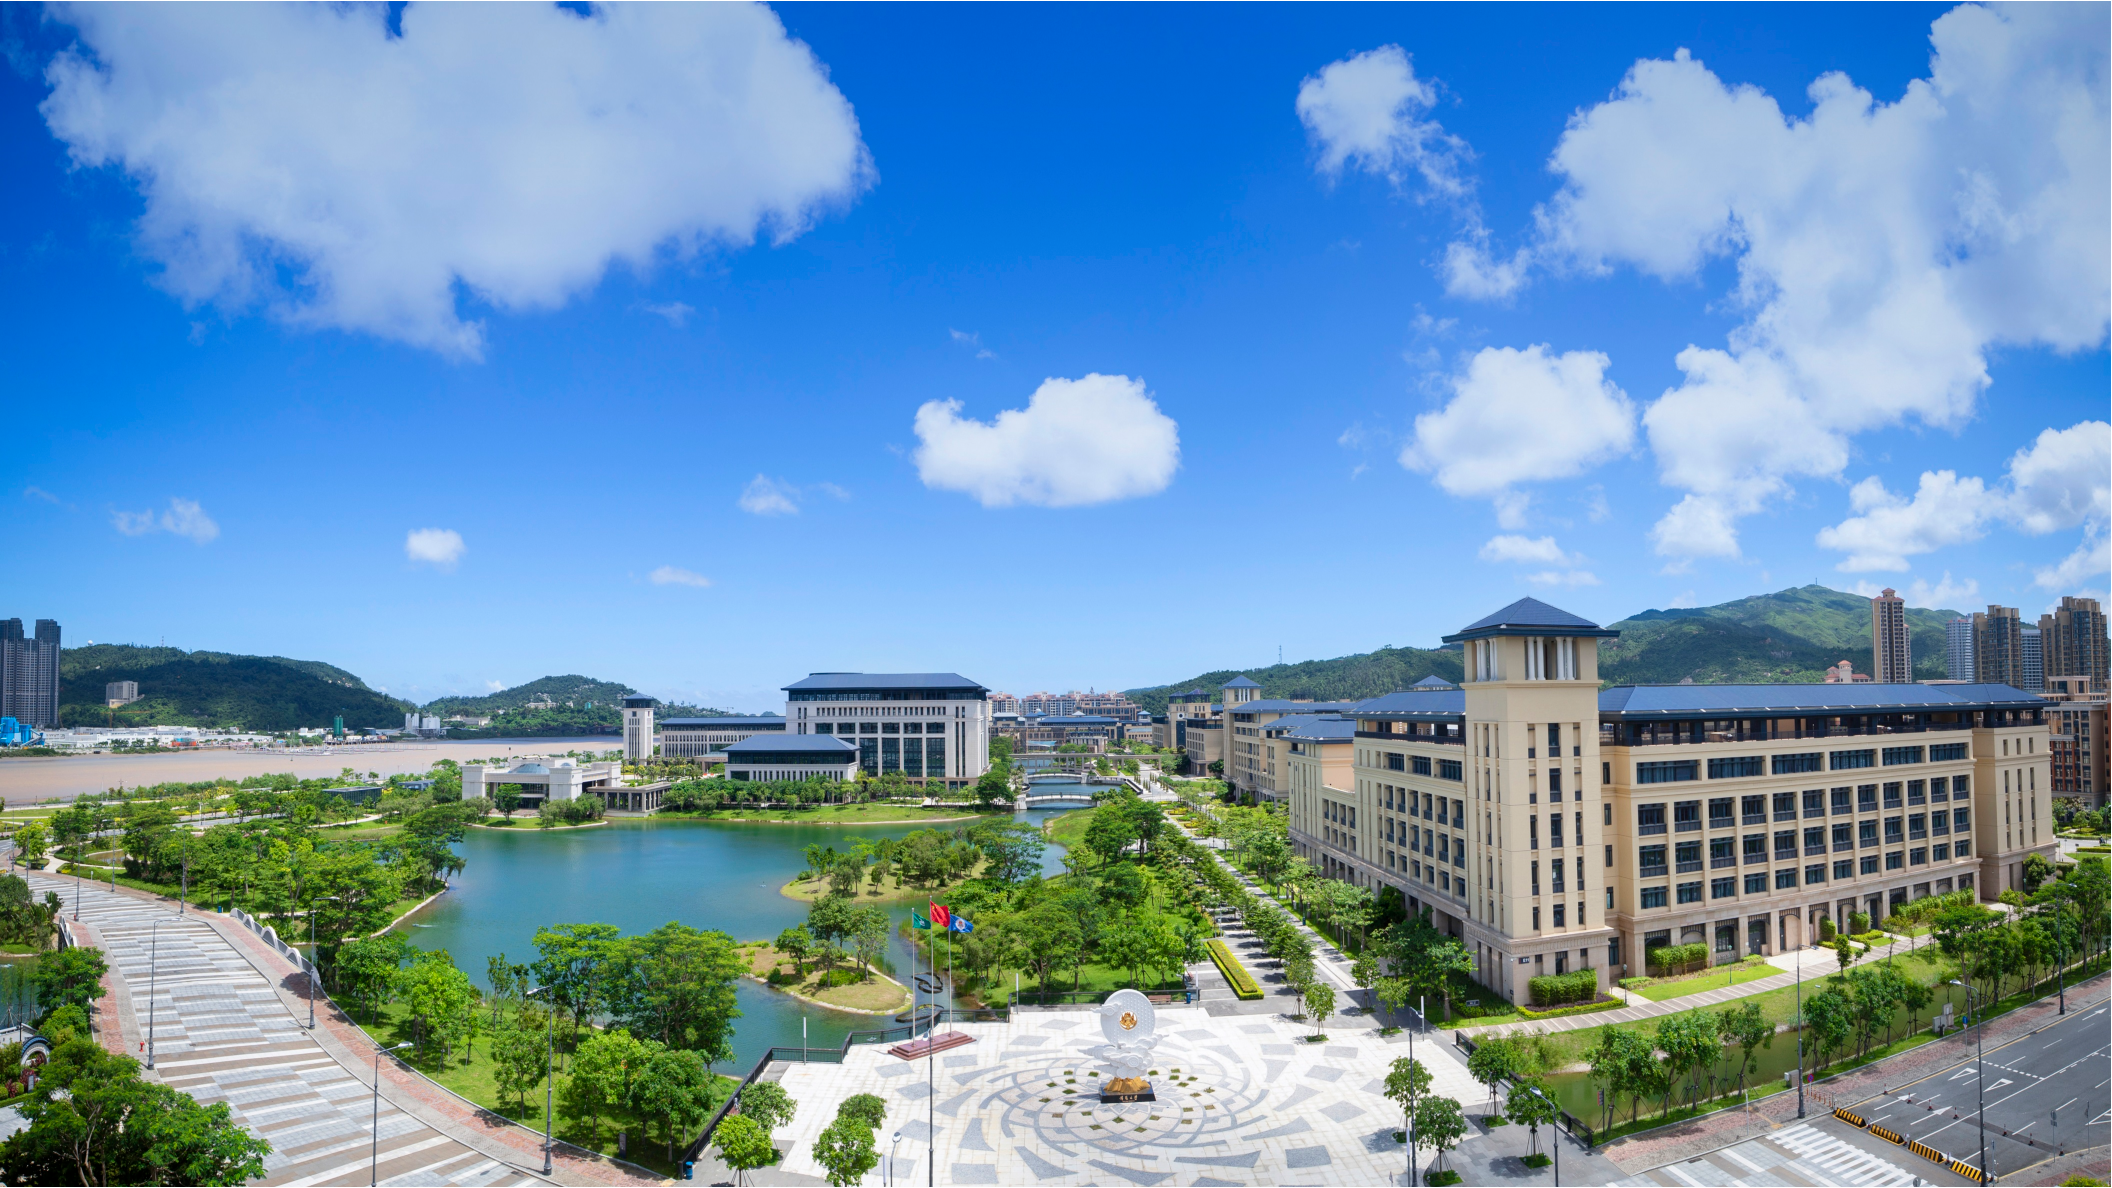
\includegraphics[height=\paperheight]{figures/UMcampus}}
\frame{

\color{white} \large
We can insert a background image like this.

	}
}
%~~~~~~~~~~~~~~~~~~~~~~~~~~~~~~~~~~~~~~~~~~~~~~~~%


%===========================================================%
% Section 2: Items, maths, citations, and figures
%===========================================================%

\section{Items, maths, citations, and figures}

%~~~~~~~~~~~~~~~~~~~~~~~~~~~~~~~~~~~~~~~~~~~~~~~~%
\begin{frame}{Bullet points and numbered items}

We can display items \alert{one by one}.

\pause

\begin{itemize}[<+->]
    \item Item \alert<2>{number one}
    \item Item \alert<3>{number two}
    \item[--] Item with a \alert<4>{dash}
\end{itemize}

\pause
Numbered items:

\begin{enumerate}[<+->]
    \item Item \alert<6>{number one}
    \item Item \alert<7>{number two}
    \item Item \alert<8>{number three}
\end{enumerate}
\end{frame}
%~~~~~~~~~~~~~~~~~~~~~~~~~~~~~~~~~~~~~~~~~~~~~~~~%



%~~~~~~~~~~~~~~~~~~~~~~~~~~~~~~~~~~~~~~~~~~~~~~~~%
\begin{frame}{A slide with {\color{UMYellow} equations}}

Probability density function of $\mathcal{N}(\mu, \sigma)$:

\begin{equation*}
f(x) = \frac{1}{\sqrt{2\pi\sigma^2}} \exp \left[ - \frac{(x-\mu)^2}{2\sigma^2} \right]
\end{equation*}

\bigskip

Posterior probability (highlight added later):
\begin{equation*}
p(\theta | x) \propto 
	\highlightcap<2->[UMGreen]{p(x | \theta)}{\footnotesize Likelihood}
	~\times~
	\highlightcap<2->[UMRed]{p(\theta)}{\footnotesize Prior}
\end{equation*}

\end{frame}
%~~~~~~~~~~~~~~~~~~~~~~~~~~~~~~~~~~~~~~~~~~~~~~~~%



%~~~~~~~~~~~~~~~~~~~~~~~~~~~~~~~~~~~~~~~~~~~~~~~~%
\begin{frame}{A slide with a {\color{UMYellow} TikZ figure}}

Security dilemma:
\begin{center}
\begin{tikzpicture}
    \node (1) [visible on=<1->] at (2,4) {\bf{\color{UMLightBlue} State A arms}};
    \node (2) [visible on=<2->,text width=3cm, align=center] at (4,2) {\bf{\color{UMRed} State B feels\\[.1em] insecure}};
    \node (3) [visible on=<3->] at (2,0) {\bf{\color{UMGreen} State B arms}};
    \node (4) [visible on=<4->,text width=3cm, align=center] at (0,2) {\bf{\color{UMYellow} State A feels\\[.1em] insecure}};
	\path (1) edge[line width=1.5, bend left = 40,visible on=<2->, color=UMLightBlue] (2);
	\path (2) edge[line width=1.5, bend left = 40,visible on=<3->, color=UMRed] (3);
	\path (3) edge[line width=1.5, bend left = 40,visible on=<4->, color=UMGreen] (4);
	\path (4) edge[line width=1.5, bend left = 40,visible on=<5->, color=UMYellow] (1);
\end{tikzpicture}
\end{center}

\end{frame}
%~~~~~~~~~~~~~~~~~~~~~~~~~~~~~~~~~~~~~~~~~~~~~~~~%




%~~~~~~~~~~~~~~~~~~~~~~~~~~~~~~~~~~~~~~~~~~~~~~~~%
\begin{frame}{A slide with a table}

\begin{table}[h!]
\centering
\caption{Security dilemma (stag hunt)}
\begin{tabular}{ccc}
			& \textbf{$\neg$Arm} & \textbf{~~Arm} \\
			\cline{2-3}
\textbf{$\neg$Arm}   & 
	\multicolumn{1}{|c|}{3,3}& 
	\multicolumn{1}{c|}{0,2} \\
			\cline{2-3}
\textbf{~~Arm}      & 
	\multicolumn{1}{|c|}{2,0}&
	\multicolumn{1}{c|}{1,1}\\
			\cline{2-3}
\end{tabular}
\label{tab:table} % Add a reference for the table
\end{table}
\end{frame}
%~~~~~~~~~~~~~~~~~~~~~~~~~~~~~~~~~~~~~~~~~~~~~~~~%


%~~~~~~~~~~~~~~~~~~~~~~~~~~~~~~~~~~~~~~~~~~~~~~~~%
\begin{frame}[fragile]\frametitle{A slide with a citation}
%[fragile] is necessary for verbatim, not for citation
 
To cite a source, we use the {\tt cite} function as follows:

{\footnotesize
\begin{verbatim}
\cite{citekeyhere}
\citep{citekeyhere} (in parentheses)
\end{verbatim}
}

Let's try citing one:
\begin{itemize}
	\item cite: \cite{fearonRationalistExplanationsWar1995} argues ...
	\item citep: ... bargaining approach \citep{fearonRationalistExplanationsWar1995}
%	\item {\scriptsize\cite{fearonRationalistExplanationsWar1995}}
\end{itemize}
 


\end{frame}
%~~~~~~~~~~~~~~~~~~~~~~~~~~~~~~~~~~~~~~~~~~~~~~~~%




%===========================================================%
% Section 3: Code and output
%===========================================================%

\section{Code and output}

%~~~~~~~~~~~~~~~~~~~~~~~~~~~~~~~~~~~~~~~~~~~~~~~~%
\begin{frame}[fragile]\frametitle{A slide with a computer code chunk}

Show some R code:

\begin{lstlisting}[language=R]
# Unload packages and clear the memory space
pacman::p_unload(pacman::p_loaded(), character.only = TRUE)
rm(list = ls())

# Load packages and data
library("tidyverse")
data("iris")

# Linear regression
fit <- lm(Sepal.Length ~ Sepal.Width + Species, data = iris)
\end{lstlisting}

\end{frame}
%~~~~~~~~~~~~~~~~~~~~~~~~~~~~~~~~~~~~~~~~~~~~~~~~%



%~~~~~~~~~~~~~~~~~~~~~~~~~~~~~~~~~~~~~~~~~~~~~~~~%
\begin{frame}{A slide with a figure}

\begin{figure}
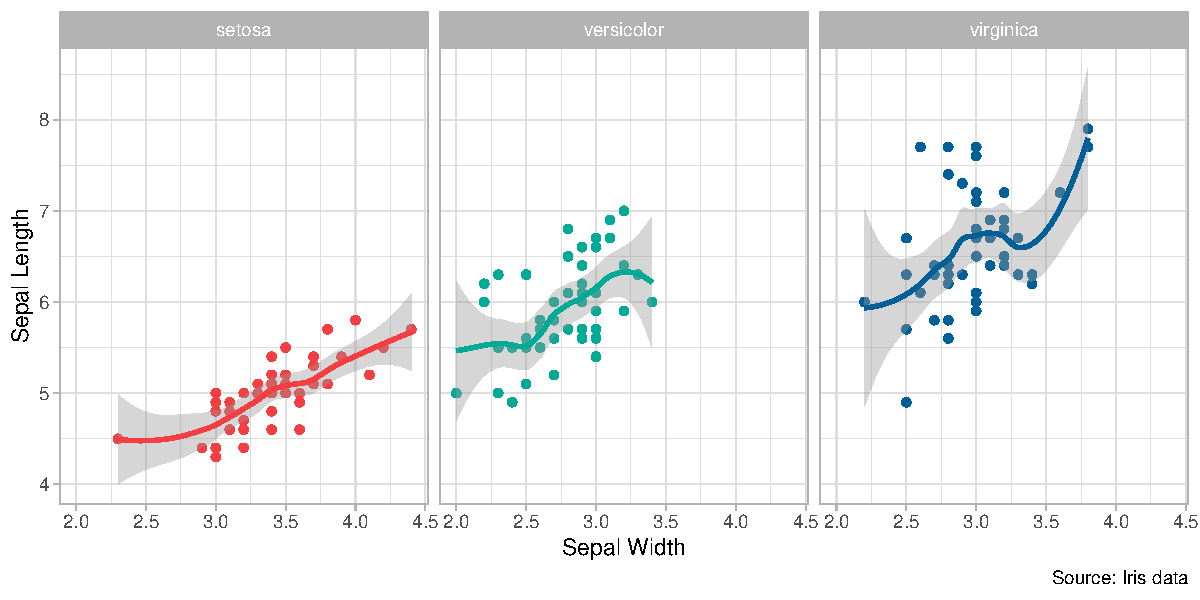
\includegraphics[width = \linewidth]{figures/iris}
\end{figure}

\end{frame}
%~~~~~~~~~~~~~~~~~~~~~~~~~~~~~~~~~~~~~~~~~~~~~~~~%

%~~~~~~~~~~~~~~~~~~~~~~~~~~~~~~~~~~~~~~~~~~~~~~~~%
\begin{frame}[fragile]\frametitle{Code to produce the figure}

\begin{lstlisting}[language=R]
# Kobe colors (brick, green, and blue)
kobe_colors <- c("#c40000", "#16832e", "#0e2f92")

# Plot: require ggplot2 and data(iris)
p <- ggplot(iris, aes(x = Sepal.Width, y = Sepal.Length, 
                      color = Species))
p + geom_point() + geom_smooth() + 
  facet_wrap(~Species) + guides(color = "none") + 
  scale_color_manual(values = kobe_colors) + 
  labs(x = "Sepal Width", y = "Sepal Length", 
       caption = "Source: Iris data") + 
  theme(
    panel.background = element_rect(fill = "transparent", 
                                    color = NA),
    plot.background = element_rect(fill = "transparent", 
                                   color = NA))
\end{lstlisting}

\end{frame}
%~~~~~~~~~~~~~~~~~~~~~~~~~~~~~~~~~~~~~~~~~~~~~~~~%


%~~~~~~~~~~~~~~~~~~~~~~~~~~~~~~~~~~~~~~~~~~~~~~~~%
\begin{frame}[fragile]\frametitle{A slide a regression table}

{\scriptsize
\begin{table}[!htbp] \centering 
  \caption{Predicting sepal length of iris}
  \label{} 
\begin{tabular}{@{\extracolsep{5pt}}lccc} 
\toprule
\\[-3ex] & \multicolumn{3}{c}{Species} \\ 
\cline{2-4} 
\\[-1.8ex] & setosa & versicolor & virginica\\ 
\midrule
 Sepal Width & 0.655$^{***}$ & 0.387$^{*}$ & 0.330$^{*}$ \\ 
  & (0.092) & (0.205) & (0.174) \\ 
 Petal Length & 0.238 & 0.908$^{***}$ & 0.946$^{***}$ \\ 
  & (0.208) & (0.165) & (0.091) \\ 
 Petal Width & 0.252 & $-$0.679 & $-$0.170 \\ 
  & (0.347) & (0.435) & (0.198) \\ 
 Constant & 2.352$^{***}$ & 1.896$^{***}$ & 0.700 \\ 
  & (0.393) & (0.507) & (0.534) \\ 
\midrule
Observations & 50 & 50 & 50 \\ 
R$^{2}$ & 0.575 & 0.605 & 0.765 \\ 
%Adjusted R$^{2}$ & 0.547 & 0.579 & 0.750 \\ 
%Residual Std. Error (df = 46) & 0.237 & 0.335 & 0.318 \\ 
%F Statistic (df = 3; 46) & 20.757$^{***}$ & 23.488$^{***}$ & 49.976$^{***}$ \\ 
\bottomrule
\textit{Note:}  & \multicolumn{3}{r}{$^{*}$p$<$0.1; $^{**}$p$<$0.05; $^{***}$p$<$0.01} \\ 
\end{tabular} 
\end{table} 

}
\end{frame}
%~~~~~~~~~~~~~~~~~~~~~~~~~~~~~~~~~~~~~~~~~~~~~~~~%



%===========================================================%
% Section 4: Reference section
%===========================================================%
\section{References}

%~~~~~~~~~~~~~~~~~~~~~~~~~~~~~~~~~~~~~~~~~~~~~~~~%
\begin{frame}[allowframebreaks] % This allows frame breaks (i.e. it creates multiple frames if the text is too long for one frame).
% \bibliographystyle{apsr} % Uncomment to change the citation style

\bibliography{literature}
\end{frame}
%~~~~~~~~~~~~~~~~~~~~~~~~~~~~~~~~~~~~~~~~~~~~~~~~%



\end{document}

